% ============================================================
% TA-IND-01 - Informe Academico Individual
% Analisis critico: HashiCorp Consul vs Netflix Eureka
% Compilar: pdflatex main -> biber main -> pdflatex main -> pdflatex main
% ============================================================
\documentclass[12pt,a4paper]{article}

\usepackage[utf8]{inputenc}
\usepackage[T1]{fontenc}
\usepackage[spanish,es-tabla]{babel}
\usepackage{lmodern}
\usepackage[margin=2.5cm]{geometry}
\usepackage{graphicx}
\usepackage{booktabs}
\usepackage{tabularx}
\usepackage{float}
\usepackage{xcolor}
\usepackage{listings}
\usepackage{csquotes}
\usepackage[backend=biber,style=ieee]{biblatex}
\usepackage{hyperref}

\addbibresource{referencias.bib}
\graphicspath{{figuras/}{../capturas/}}

\lstset{
  basicstyle=\ttfamily\footnotesize,
  breaklines=true,
  frame=single,
  backgroundcolor=\color{gray!8}
}

\hypersetup{colorlinks=true, linkcolor=black, urlcolor=blue, citecolor=blue}

% ------------------------------------------------------------
\begin{document}

% ======================= CARATULA ===========================
\begin{titlepage}
  \centering
  {\Large\bfseries Universidad Técnica Estatal de Quevedo\par}
  \vspace{0.3cm}
  {\large Facultad de Ciencias de la Computación\par}
  \vspace{0.2cm}
  {\large Carrera de Ingeniería de Software\par}
  \vspace{1.5cm}
  {\large Asignatura: Sistemas Distribuidos\par}
  \vspace{0.3cm}
  {\large Actividad: TA-IND-01 --- Informe Académico Individual\par}
  \vspace{2cm}
  {\LARGE\bfseries Análisis crítico de HashiCorp Consul\\[0.2cm] comparado con Netflix Eureka\par}
  \vspace{2cm}
  {\large \textbf{Estudiante:} Leonel Leonidas Zambrano Triviño\par}
  \vspace{0.3cm}
  {\large \textbf{Paralelo:} B\par}
  \vspace{0.3cm}
  {\large \textbf{Docente:} Ing. Gleiston Cicerón Guerrero Ulloa\par}
  \vspace{0.3cm}
  {\large \textbf{Fecha:} 15 de noviembre de 2026\par}
  \vfill
  {\small \textbf{Repositorio:} \url{https://github.com/lzambranot6-sys/TA-IND-01-Consul-vs-Eureka}\par}
\end{titlepage}

% ======================= RESUMEN ============================
\begin{abstract}
En este informe se analiza HashiCorp Consul, un sistema de descubrimiento de servicios (\textit{service discovery}) usado en arquitecturas de microservicios, y se compara con Netflix Eureka, que resuelve el mismo problema con un enfoque diferente. El análisis aplica los conceptos de la Unidad 1: transparencias de distribución, teorema CAP y su extensión PACELC, modelos de comunicación y tolerancia a fallos. Para respaldar el análisis se levantó un clúster local de tres servidores de Consul con Docker y se realizaron dos experimentos: la caída del nodo líder y la pérdida del quórum. En el primero, el clúster eligió un nuevo líder mediante Raft y el nodo caído se reincorporó y se puso al día sin intervención manual. En el segundo, con un solo servidor activo, Consul rechazó las escrituras y las lecturas normales, y solo respondió a las lecturas en modo \textit{stale}. Esto confirma que Consul prioriza la consistencia ante una partición (CP), mientras que Eureka prioriza la disponibilidad (AP). Se concluye que Consul es adecuado cuando la exactitud del registro es crítica, pero su consenso limita la escalabilidad y lo vuelve indisponible si se pierde la mayoría.
\end{abstract}

\newpage
\tableofcontents
\newpage

% ======================= INTRODUCCION =======================
\section{Introducción}
Las aplicaciones modernas ya no se construyen como un solo bloque (monolito), sino como un conjunto de microservicios pequeños e independientes que se comunican por la red. La migración de monolitos hacia microservicios es hoy un tema central de la ingeniería de software \cite{abgaz2023decomposition}. Este cambio trae un problema nuevo: los servicios se crean, se destruyen y cambian de máquina constantemente, por lo que su dirección IP y su puerto no son fijos. Un servicio que necesita comunicarse con otro no puede tener esa dirección escrita en su código.

La solución a este problema es el descubrimiento de servicios (\textit{service discovery}), que consiste en detectar automáticamente los microservicios dentro de la infraestructura \cite[p.~90254]{haindl2024security}. Para esto existe un registro central donde cada servicio se anota al iniciar y donde los demás preguntan dónde encontrarlo.

HashiCorp Consul es una de las herramientas más usadas para este fin. Además del registro de servicios, ofrece verificación de salud (\textit{health checks}) y un almacén clave-valor. Un ejemplo de su uso a gran escala es Roblox, una plataforma con unos 50 millones de jugadores diarios, que usa Consul para descubrimiento de servicios, verificación de salud, bloqueo de sesiones y almacenamiento clave-valor \cite{roblox2022outage}.

Se eligió Consul porque representa un diseño que prioriza la consistencia, lo que permite contrastarlo con Netflix Eureka, que resuelve el mismo problema priorizando la disponibilidad. Esta diferencia permite aplicar de forma concreta el teorema CAP y su extensión PACELC.

% ======================= ARQUITECTURA =======================
\section{Arquitectura del sistema}
Un clúster de Consul se organiza por centros de datos (\textit{datacenters}). Dentro de cada uno existen dos tipos de agentes:

\begin{itemize}
  \item \textbf{Servers}: normalmente 3 o 5. Guardan el estado del clúster (el catálogo de servicios y el almacén clave-valor) y participan en el algoritmo de consenso Raft. Uno de ellos es elegido \textbf{líder} y los demás son \textbf{seguidores} (\textit{followers}).
  \item \textbf{Clients}: se ejecuta uno por cada máquina donde corren microservicios. No guardan el estado global ni votan; registran los servicios locales, ejecutan sus verificaciones de salud y reenvían las consultas a los servers.
\end{itemize}

Los componentes se comunican por tres canales distintos, como se observa en la Figura~\ref{fig:arquitectura}:

\begin{itemize}
  \item \textbf{Raft (RPC, puerto 8300)}: solo entre servers. Toda escritura pasa por el líder y se confirma cuando la mayoría de servers la ha replicado.
  \item \textbf{Gossip (puerto 8301)}: entre todos los nodos. Cada nodo intercambia mensajes con otros elegidos al azar para saber quién sigue vivo.
  \item \textbf{HTTP y DNS (puertos 8500 y 8600)}: es la interfaz que usan los microservicios y los operadores para registrar y consultar servicios.
\end{itemize}

El diagrama final es una evolución del esquema hecho a mano al inicio del trabajo (Anexo A). En el esquema inicial solo aparecían los tres servers y el cliente; en el diagrama final se agregaron los agentes cliente, los microservicios y la diferencia entre el canal de Raft y el de gossip.

\begin{figure}[H]
  \centering
  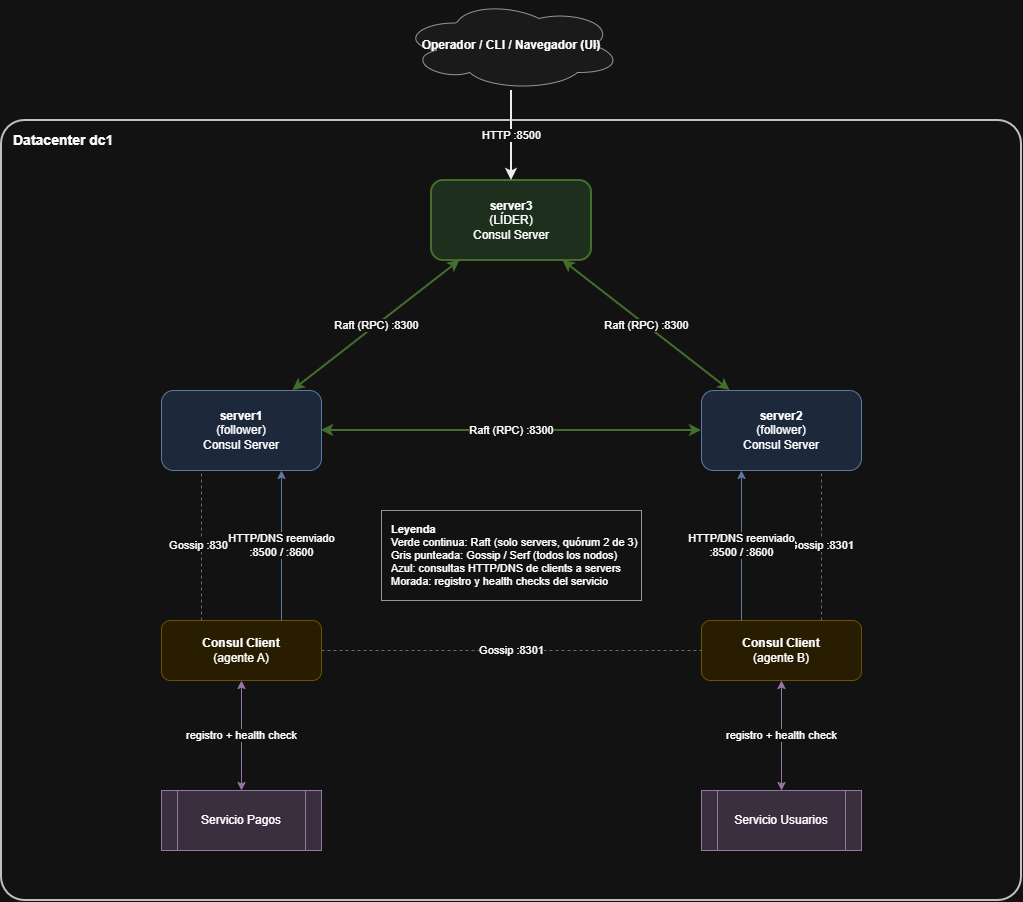
\includegraphics[width=0.9\textwidth]{arquitectura-consul.png}
  \caption{Arquitectura de un datacenter de Consul (elaboración propia).}
  \label{fig:arquitectura}
\end{figure}

% ======================= ANALISIS U1 ========================
\section{Análisis con los conceptos de la Unidad 1}

\subsection{Transparencias de distribución}
\begin{itemize}
  \item \textbf{Acceso}: los servicios consultan a Consul siempre de la misma forma (HTTP o DNS), sin importar en qué server está el dato.
  \item \textbf{Ubicación}: un microservicio pide, por ejemplo, \texttt{pagos.service.consul} y recibe la dirección actual, sin conocer de antemano la IP del otro servicio.
  \item \textbf{Migración y reubicación}: si un servicio se mueve a otra máquina, se vuelve a registrar con su nueva dirección y los consumidores lo encuentran sin cambiar su código.
  \item \textbf{Replicación}: el estado está copiado en los tres servers, pero el cliente no lo nota; ve un único registro.
  \item \textbf{Concurrencia}: varias escrituras simultáneas se ordenan en el registro (\textit{log}) de Raft, por lo que el cliente no tiene que coordinarse con otros.
  \item \textbf{Fallos}: es parcial. En el experimento 1 la caída del líder fue invisible para el usuario porque se eligió otro automáticamente. Pero en el experimento 2, al perder la mayoría, el cliente sí recibió un error. Consul oculta la caída de una minoría de servers, no la de la mayoría.
\end{itemize}

\subsection{CAP y PACELC}
Consul usa el algoritmo de consenso Raft: todas las escrituras pasan por el líder y solo se confirman cuando una mayoría (quórum) de servers las ha copiado. Con tres servers el quórum es dos.

\textbf{Con partición (P)}: si un server queda aislado sin mayoría, no puede aceptar escrituras ni elegirse líder. Consul prefiere no responder antes que arriesgarse a tener datos distintos en cada nodo; por tanto elige \textbf{consistencia} y sacrifica disponibilidad. Esto se comprobó en el experimento 2, donde la escritura falló con el error \texttt{No cluster leader}. Según la clasificación CAP, Consul es un sistema \textbf{CP}.

\textbf{Sin partición (E)}: en funcionamiento normal también prioriza la consistencia, porque por defecto las lecturas las responde el líder. Sin embargo, Consul ofrece varios modos de consistencia para las lecturas; en el modo \textit{stale} cualquier server puede responder, sea o no el líder \cite{hashicorp_consistency}. Así se gana menor latencia a cambio de datos que podrían estar desactualizados.

Por eso, en términos de PACELC, Consul es \textbf{PC/EC} por defecto, pero permite que el cliente elija latencia (\textbf{EL}) en lecturas puntuales. Eureka, en cambio, es \textbf{PA/EL}: siempre responde, aunque los datos sean antiguos.

\subsection{Modelos de comunicación}
Consul usa un modelo \textbf{híbrido}:
\begin{itemize}
  \item \textbf{Cliente-servidor}: los microservicios hablan con su agente cliente, y este reenvía las consultas a los servers mediante HTTP o DNS.
  \item \textbf{Peer-to-peer}: el protocolo de gossip conecta a todos los nodos por igual, sin un nodo central, para compartir quién pertenece al clúster y quién está vivo.
\end{itemize}

En cuanto a la sincronía, las consultas HTTP y la replicación de Raft son \textbf{sincrónicas}: quien pregunta espera la respuesta. El gossip es \textbf{asincrónico}: los mensajes se propagan poco a poco por la red sin que nadie espere una confirmación. Los mecanismos usados son \textbf{RPC} entre servers, \textbf{HTTP/REST} y \textbf{DNS} hacia los clientes, y mensajes de gossip entre todos los nodos. En el experimento se vio que cada canal usa su propio puerto: 8300 para Raft y 8301 para gossip.

\subsection{Tolerancia a fallos}
\textbf{Qué fallos soporta}: un clúster de 3 servers soporta la caída de 1, y uno de 5 soporta la caída de 2, porque siempre debe quedar una mayoría.

\textbf{Cómo los detecta}: mediante el gossip, cada nodo comprueba periódicamente si los demás responden; además, los agentes cliente ejecutan verificaciones de salud sobre cada servicio registrado. Esta información de salud también alimenta a herramientas de monitoreo: por ejemplo, Prometheus se integra con varias opciones de descubrimiento de servicios \cite[p.~72019]{faseeha2025observability}.

\textbf{Cómo se recupera}: si cae el líder, los seguidores dejan de recibir sus mensajes y convocan una elección; el nodo que obtiene la mayoría de votos se convierte en el nuevo líder. Este esquema de consenso basado en un líder también aparece en algoritmos como PBFT, donde un nodo líder se elige para coordinar \cite{islam2023consensus}. Cuando un server caído vuelve, Consul lo reincorpora primero sin voto y, cuando está estable, le da voto; mientras tanto el nodo copia lo que se perdió.

\textbf{Incidente real}: en octubre de 2021, Roblox sufrió una interrupción de 73 horas causada por problemas en su clúster de Consul, del que dependían muchos de sus servicios \cite{roblox2022outage}. Meses antes habían actualizado Consul para usar una nueva función de \textit{streaming}, y bajo carga alta el rendimiento del clúster se degradó; los intentos iniciales de recuperarlo, incluso cambiando todos los servers por máquinas más potentes, no funcionaron. Este caso muestra que, aunque Consul tolera la caída de nodos, si el propio sistema de descubrimiento falla, arrastra a todos los servicios que dependen de él.

% ======================= EXPERIMENTACION ====================
\section{Experimentación propia}

\subsection{Entorno}
Los experimentos se realizaron en una laptop con Windows y Docker Desktop. Se levantó un clúster de tres servers de Consul (versión 1.20.6) con Docker Compose; cada server corre en su propio contenedor. Los archivos y las salidas completas están en la carpeta \texttt{experimento/consul} del repositorio.

\begin{figure}[H]
  \centering
  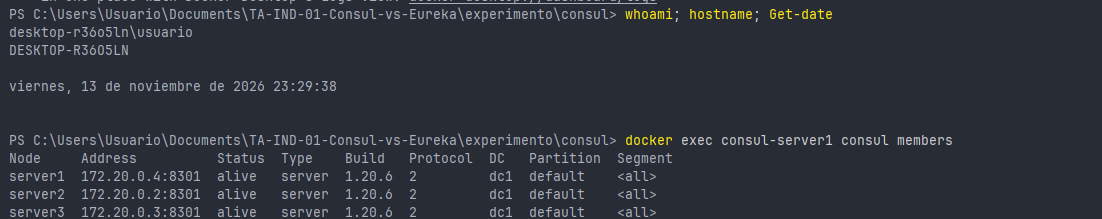
\includegraphics[width=0.85\textwidth]{01-consul-members.png}
  \caption{Clúster de 3 servers activos (\texttt{consul members}).}
\end{figure}

\subsection{Experimento 1: caída del líder}
\textbf{Objetivo}: comprobar si el clúster sigue funcionando cuando se cae el líder y cómo se reincorpora el nodo caído.

\textbf{Procedimiento}: se consultó el estado de Raft con \texttt{consul operator raft list-peers}, se detuvo el contenedor del líder con \texttt{docker stop}, se volvió a consultar y finalmente se encendió de nuevo.

\textbf{Resultado e interpretación}: antes de la caída, server2 era el líder y los tres nodos tenían el mismo \textit{Commit Index}, es decir, estaban sincronizados. Al detener server2, los otros dos eligieron a server3 como nuevo líder y el clúster siguió aceptando operaciones (el \textit{Commit Index} subió de 191 a 224). Esto demuestra la tolerancia a fallos y la transparencia de fallos. Al reincorporarse, server2 apareció primero sin voto (\textit{Voter = false}) y luego como votante, con el mismo \textit{Commit Index} que los demás. Además, server3 siguió como líder: la vuelta del nodo no provocó una nueva elección.

\begin{figure}[H]
  \centering
  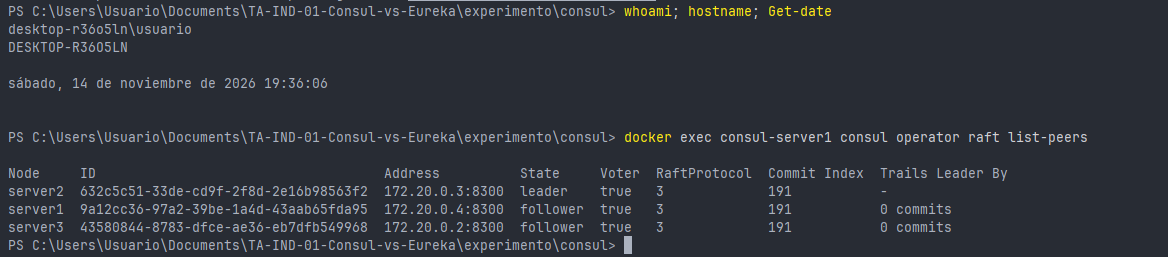
\includegraphics[width=0.85\textwidth]{04-antes-caida-lider.png}
  \caption{Estado de Raft antes de la caída: server2 es líder.}
\end{figure}

\begin{figure}[H]
  \centering
  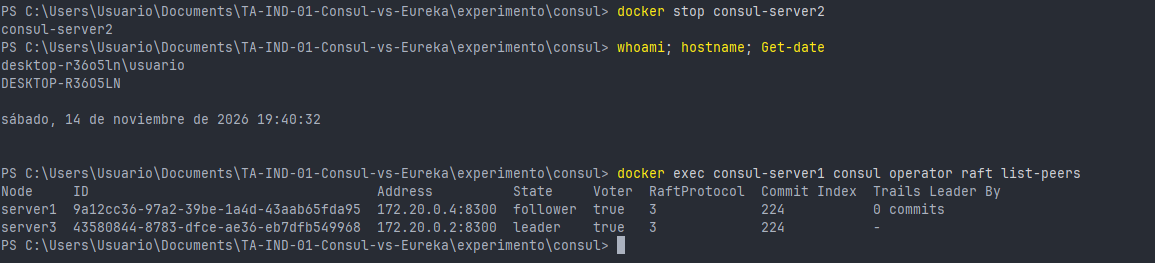
\includegraphics[width=0.85\textwidth]{05-asignacion-lider.png}
  \caption{Tras detener server2, server3 es elegido nuevo líder.}
\end{figure}

\begin{figure}[H]
  \centering
  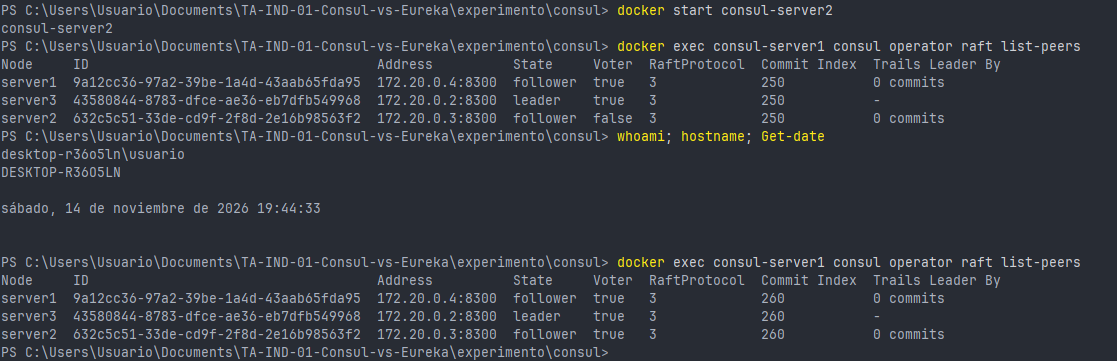
\includegraphics[width=0.85\textwidth]{06-reincorporacion-server2.png}
  \caption{Reincorporación de server2: primero sin voto, luego votante.}
\end{figure}

\subsection{Experimento 2: pérdida de quórum}
\textbf{Objetivo}: comprobar qué prioriza Consul cuando pierde la mayoría de servers: consistencia o disponibilidad.

\textbf{Procedimiento}: se guardó un valor en el almacén clave-valor, se apagaron de golpe dos servers con \texttt{docker kill} (simulando una caída real, sin aviso) y desde el único server vivo se intentó escribir, leer de forma normal y leer en modo \textit{stale}.

\textbf{Resultado e interpretación}: la escritura y la lectura normal fallaron con el error \texttt{No cluster leader}; la lectura con \texttt{-stale} sí respondió con el valor guardado antes de la caída. Esto confirma que, ante una partición, Consul elige consistencia (CP), pero permite al cliente pedir disponibilidad a cambio de datos que podrían estar desactualizados, que es el matiz que describe PACELC. Al encender los servers de nuevo, el quórum se recuperó y la lectura normal volvió a funcionar.

\begin{figure}[H]
  \centering
  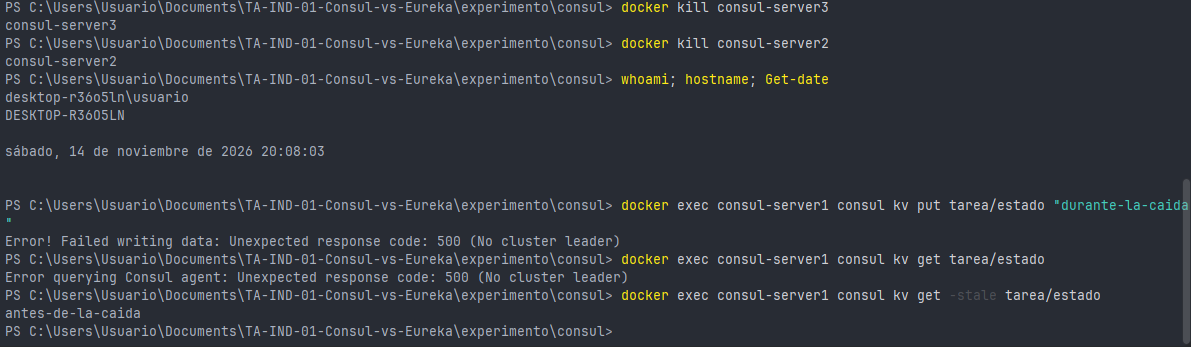
\includegraphics[width=0.85\textwidth]{08-sin-quorum.png}
  \caption{Sin quórum: escritura y lectura normal fallan; la lectura \texttt{-stale} responde.}
\end{figure}

% ======================= ENTORNO ============================
\section{Ejemplos del entorno del estudiante}
\subsection{SGA de la UTEQ}
Ahora mismo, domingo 15 de noviembre, entre al sga y estaba lento, para todo.

\subsection{WhatsApp}
Me pasaba que en el WhatsApp web cuando mandaba un mensaje, no se iba, y si tenia internet, en mi celular si se podia, pero en WhatsApp web, no, nunca supe que pasaba.


% ======================= COMPARATIVO ========================
\section{Análisis comparativo}

\begin{table}[H]
  \centering
  \caption{Comparación entre Consul y Eureka según criterios de la Unidad 1.}
  \label{tab:comparacion}
  \begin{tabularx}{\textwidth}{>{\raggedright\arraybackslash}p{3.2cm}XX}
    \toprule
    \textbf{Criterio} & \textbf{Consul} & \textbf{Eureka} \\
    \midrule
    Clasificación CAP & CP & AP \\
    PACELC & PC/EC (lecturas \textit{stale} opcionales) & PA/EL \\
    Coordinación & Raft con líder y quórum & Réplicas iguales sin líder \\
    Comunicación & HTTP/DNS, RPC y gossip (híbrido) & REST/HTTP y replicación entre pares \\
    Detección de fallos & Gossip (SWIM) y health checks & Heartbeats cada 30 s, expiración a 90 s \\
    Comportamiento sin mayoría & Rechaza escrituras (verificado en exp. 2) & Sigue respondiendo; \textit{self-preservation} \\
    Escalabilidad del consenso & Limitada a 3--5 servers votantes & Sin consenso, escala añadiendo réplicas \\
    \bottomrule
  \end{tabularx}
\end{table}

La Tabla~\ref{tab:comparacion} muestra que la diferencia de fondo entre ambos sistemas es qué hacen cuando la red falla. Consul usa consenso con líder y quórum, por lo que su registro siempre es consistente, pero si se pierde la mayoría deja de aceptar escrituras, como se comprobó en el experimento 2. Eureka no usa consenso: sus réplicas son iguales y se copian los datos entre sí, por lo que siempre responde, aunque la información pueda estar desactualizada. Su modo de autopreservación (\textit{self-preservation}) evita borrar servicios cuando de repente dejan de llegar muchos latidos, porque asume que el problema es de la red y no de los servicios.

En la práctica, Eureka se comporta siempre como las lecturas \textit{stale} de Consul. Consul conviene cuando es grave enviar una petición a una instancia que ya no existe o cuando también se necesita un almacén clave-valor consistente. Eureka conviene cuando es preferible que el sistema siga respondiendo aunque algún dato esté viejo, y cuando la aplicación ya está construida con Spring Cloud.

% ======================= POSTURA CRITICA ====================
\section{Postura crítica}
\textbf{Fortalezas}: Consul garantiza que todos los servers tengan la misma información y se recupera solo ante la caída de una minoría de nodos, como se vio en el experimento 1. Además combina varias funciones (registro, salud, clave-valor) en una sola herramienta.

\textbf{Limitaciones}: su principal debilidad es que, sin quórum, deja de aceptar escrituras; el sistema de descubrimiento, del que dependen todos los demás servicios, se vuelve un punto crítico. El caso de Roblox muestra que una falla en Consul puede detener una plataforma completa durante días \cite{roblox2022outage}. Además, el consenso no escala a muchos nodos votantes: en algoritmos como PBFT, la sobrecarga de difundir bloques y votos impide escalar más allá de unas decenas de validadores \cite{islam2023consensus}. Por eso Consul limita los servers a 3 o 5 y deja al resto como clientes sin voto.

\textbf{Costos}: mantener varias réplicas y agentes en cada máquina consume más recursos; en general, los microservicios implican demandas importantes de energía para alcanzar los niveles de rendimiento y disponibilidad deseados \cite{araujo2024energy}.

\textbf{Seguridad}: el registro de servicios es un punto atractivo para atacantes, ya que quien lo controle puede redirigir las peticiones; el descubrimiento de servicios forma parte de los temas de seguridad en la comunicación entre microservicios \cite{haindl2024security}.

\textbf{Cuándo no usar Consul}: en sistemas donde es preferible responder siempre, aunque sea con datos viejos, y donde una caída del registro sería peor que un dato desactualizado. En esos casos un diseño AP como Eureka es más adecuado. Tampoco conviene para equipos pequeños que no pueden operar un clúster de varios servers.

% ======================= CONCLUSIONES =======================
\section{Conclusiones}
\begin{itemize}
  \item En el experimento 1, al detener al líder, el clúster eligió otro y siguió funcionando sin intervención manual: Consul tolera la caída de una minoría de servers.
  \item Un server que vuelve se reincorpora primero sin voto y se pone al día solo, lo que evita que un nodo inestable altere las elecciones.
  \item En el experimento 2, sin quórum, Consul rechazó escrituras y lecturas normales: ante una partición prioriza la consistencia y es CP.
  \item La lectura en modo \textit{stale} sí respondió, lo que muestra que Consul permite cambiar consistencia por disponibilidad o latencia en lecturas puntuales (PACELC).
  \item Frente a Eureka, Consul es la mejor opción cuando la exactitud del registro importa más que responder siempre; Eureka lo es en el caso contrario.
\end{itemize}

% ======================= DECLARACION IA =====================
\section*{Declaración de uso de inteligencia artificial}
Se utilizó Claude (Anthropic, modelo Claude Opus 5.5) para: elegir el sistema a analizar entre los que no estaban tomados, entender los conceptos de Consul y Eureka, guiar los comandos de Docker para levantar el clúster y los experimentos, generar una primera versión del diagrama de arquitectura a partir de mi esquema a mano, y proponer una plantilla y un texto base para el informe en LaTeX. Lo obtenido se verificó ejecutando yo mismo los experimentos en mi equipo, comparando las salidas con lo explicado, abriendo cada DOI para comprobar los datos de las referencias, leyendo los fragmentos citados y reescribiendo el texto con mis propias palabras.

% ======================= REFERENCIAS ========================
\printbibliography[title={Referencias}]

% ======================= ANEXOS =============================
\newpage
\appendix
\section{Esquema inicial a mano}
\begin{figure}[H]
  \centering
  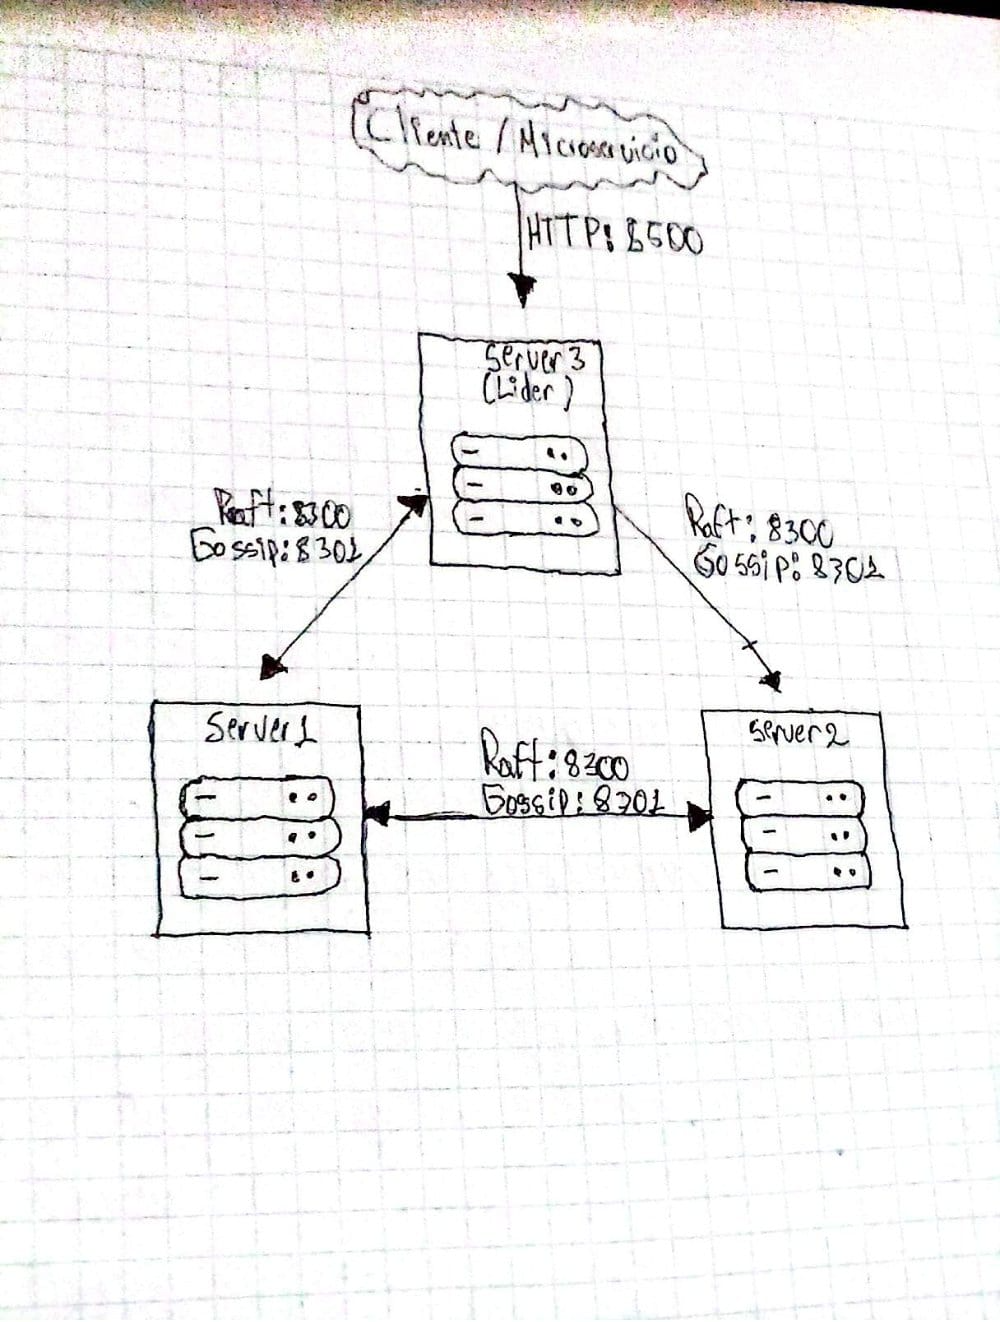
\includegraphics[width=0.7\textwidth]{anexo-A-esquema-a-mano.png}
  \caption{Primer bosquejo de la arquitectura, dibujado a mano.}
\end{figure}

\section{Capturas de lectura de las fuentes}
\begin{figure}[H]
  \centering
  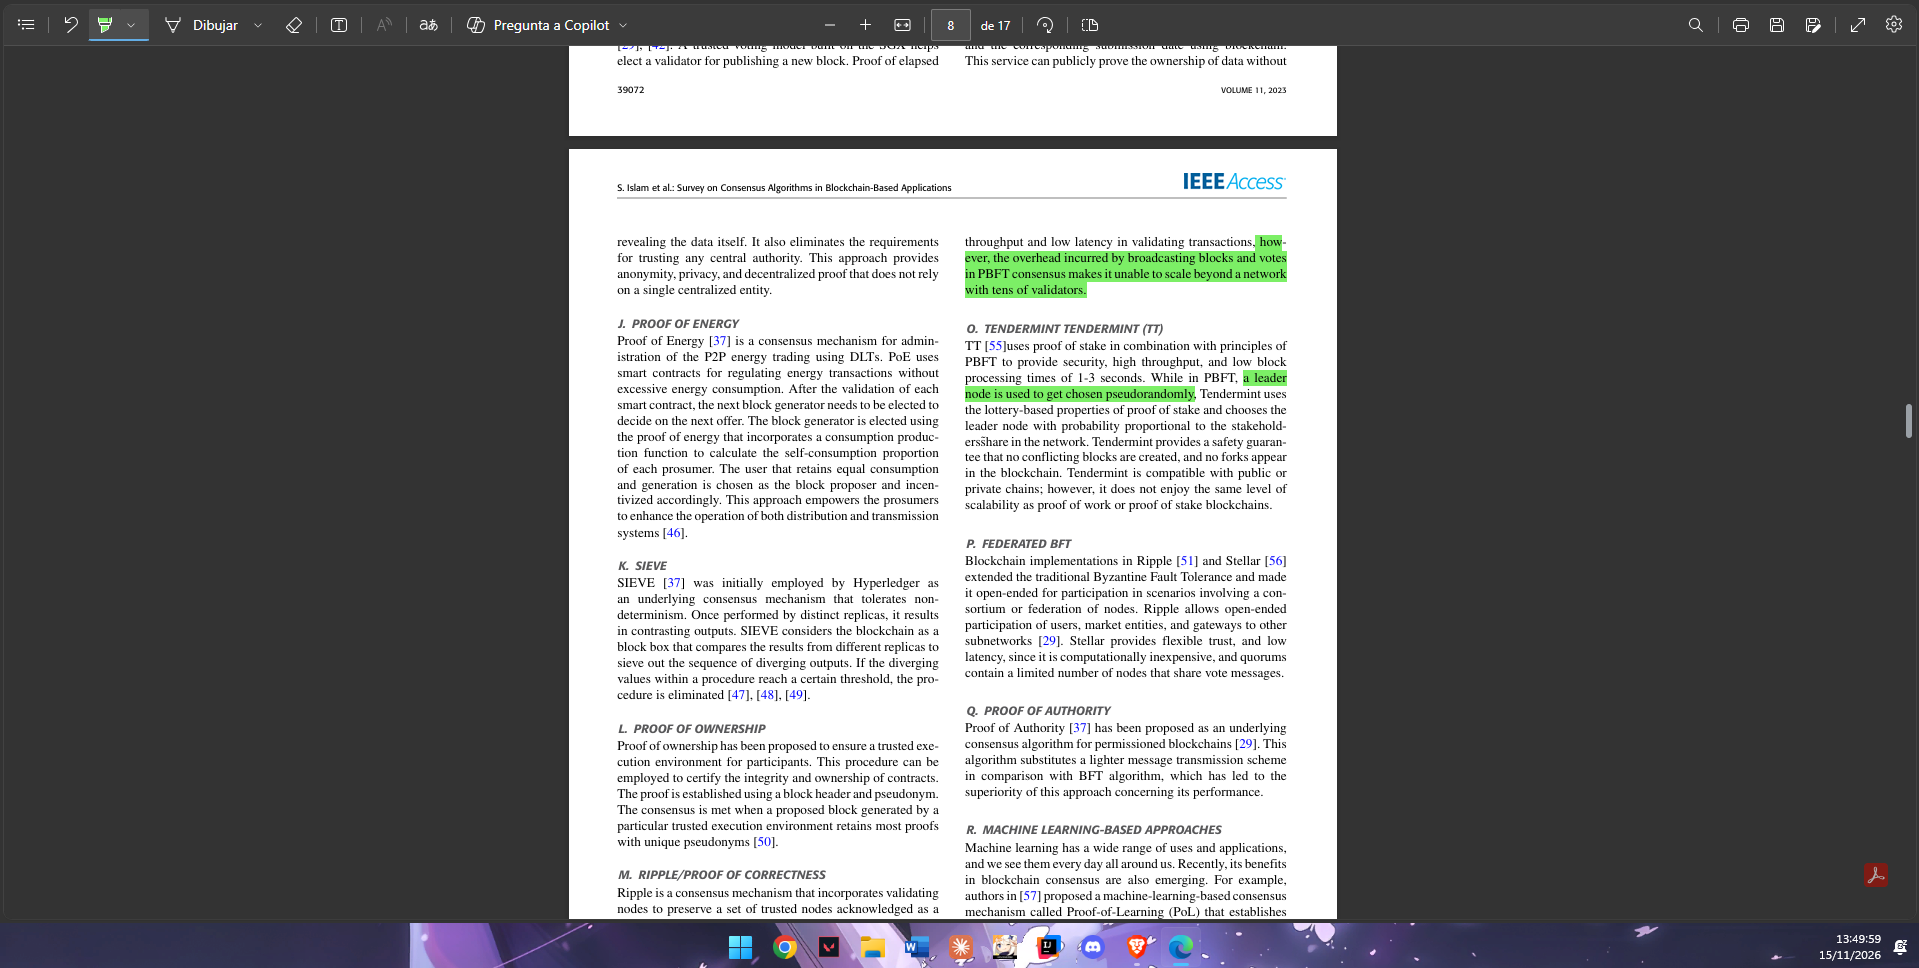
\includegraphics[width=0.9\textwidth]{anexo-B-1-islam.png}
  \caption{Lectura de Islam et al. \cite{islam2023consensus}.}
\end{figure}
\begin{figure}[H]
  \centering
  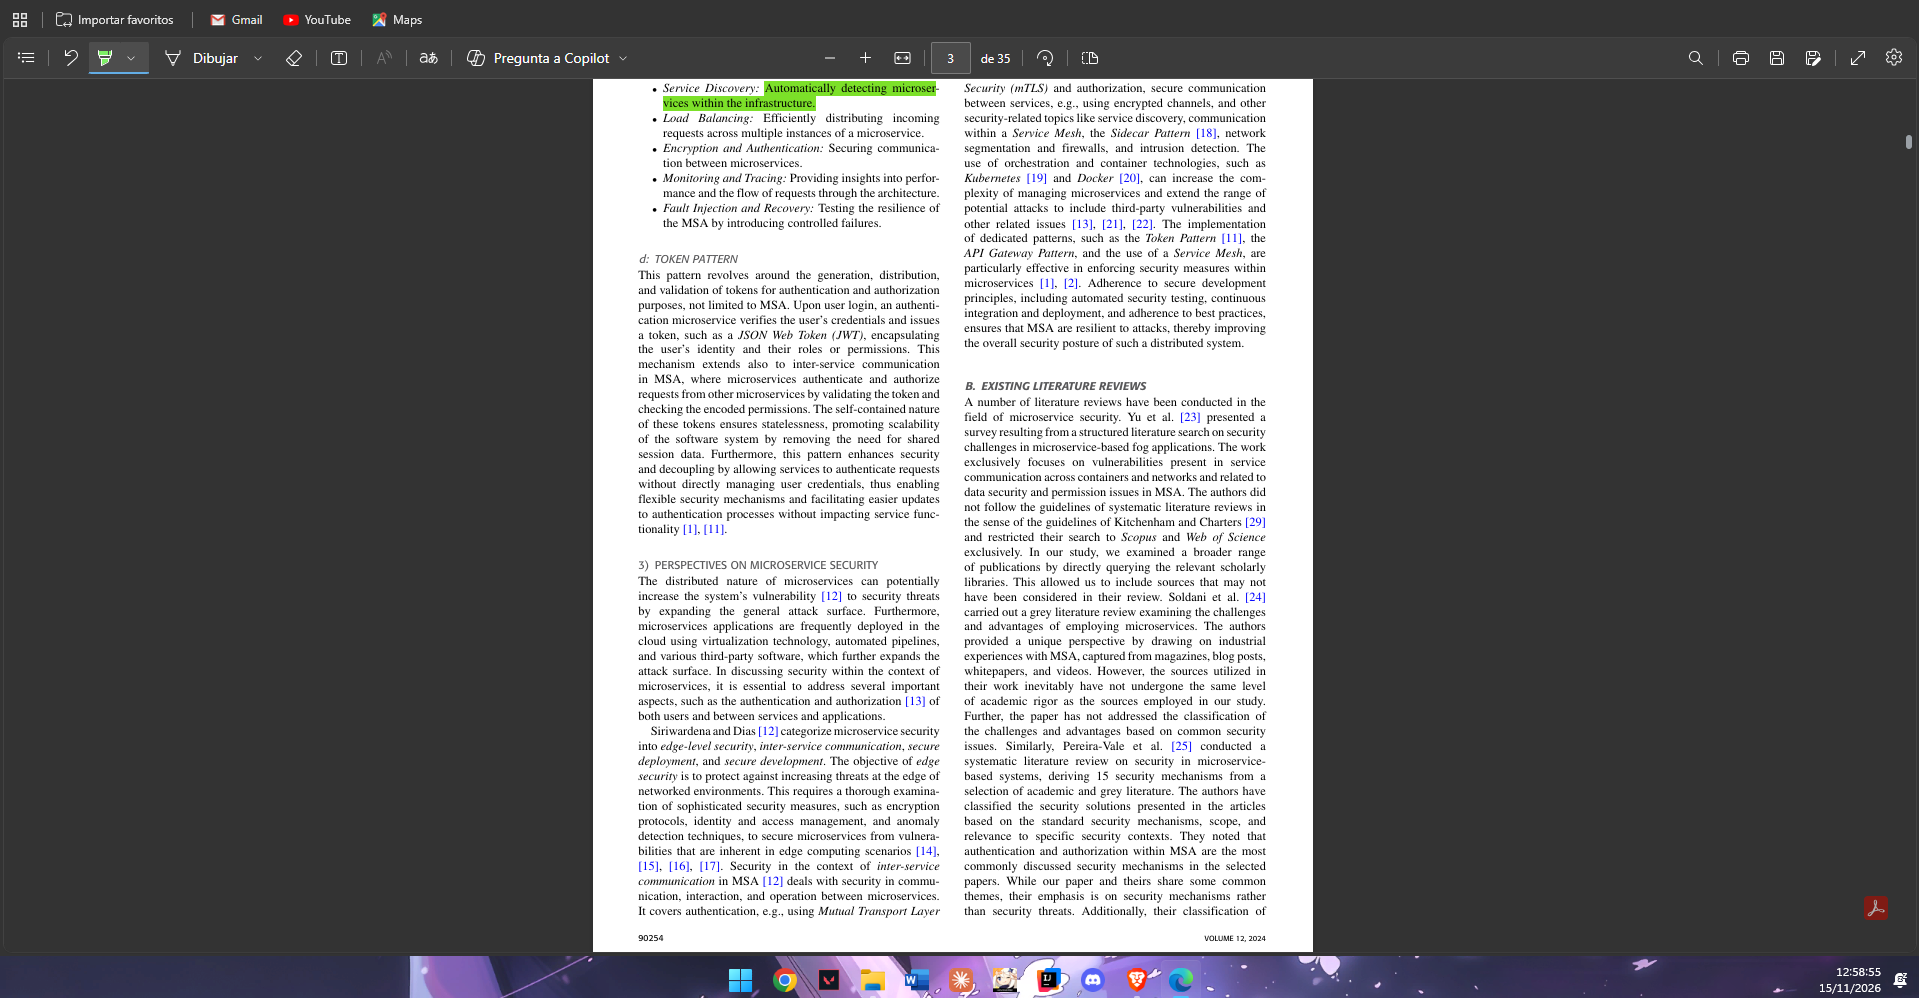
\includegraphics[width=0.9\textwidth]{anexo-B-2-haindl.png}
  \caption{Lectura de Haindl et al. \cite{haindl2024security}, p. 90254.}
\end{figure}
\begin{figure}[H]
  \centering
  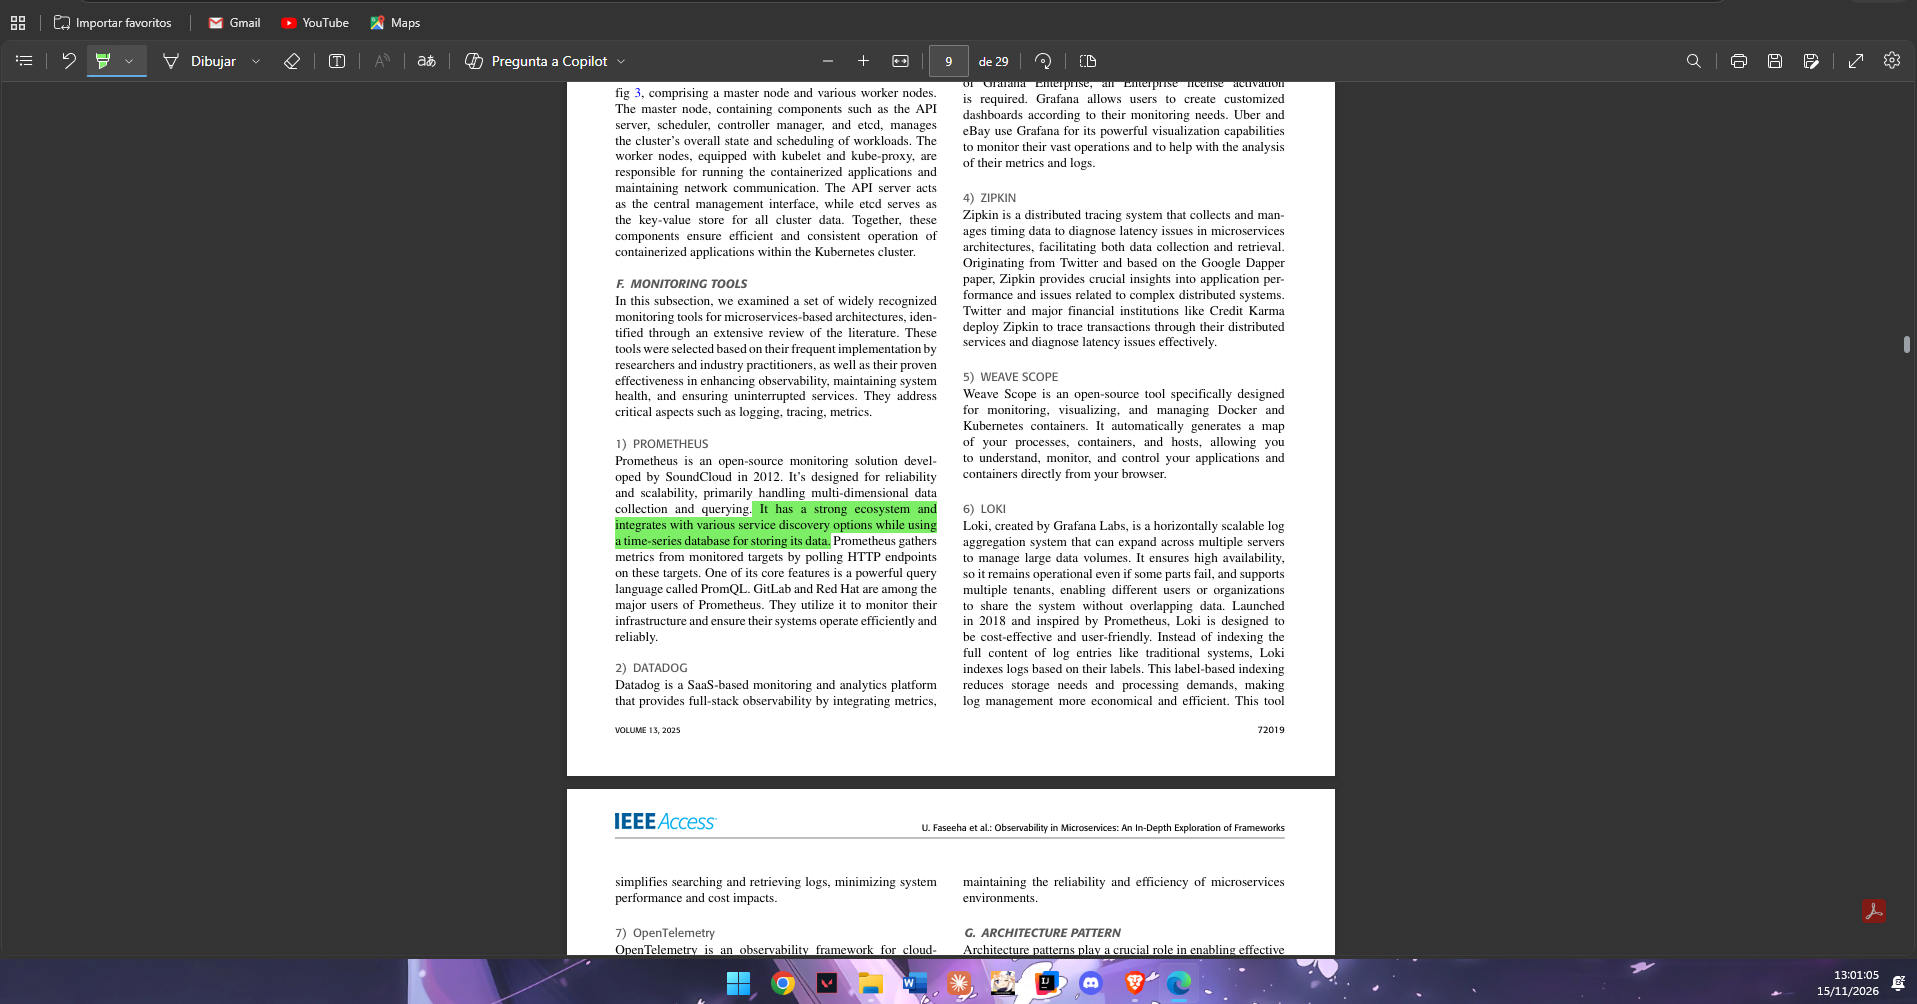
\includegraphics[width=0.9\textwidth]{anexo-B-3-faseeha.png}
  \caption{Lectura de Faseeha et al. \cite{faseeha2025observability}, p. 72019.}
\end{figure}

\end{document}
